\section{Dataset}
For our work we collected posts from Vine social network, about top 100 popular posts over all and also over specific channel categories. We collected the metadata every 6 hours to make sure there is minimal overlap in rankings and we continued this exercise for over a month. Finally we filtered all the uniques posts out and collected the actual vine mp4 files. In total we have 16504 unique vine clips collected over a month that ranked in the top 100 posts across vine. We also store the individual post metadata and the profile of the post creator. Some statistics for our dataset are as follows 
\par
\begin{center}
\begin{tabular}{ |c|c|c| } 
 \hline
 Parameter & mean Value & Median Value \\ 
 \hline
 Reposts & 1558 & 552 \\ 
 Likes & 5754 & 2193 \\ 
 Loops & 205504 & 76895 \\ 
 \hline
\end{tabular}
\end{center}
\par
From the statistics of reactions to vines, it seems loops or the number of times a video is replayed is not necessarily a good measure to quantify popularity. However the likes and repost count could act as a good descriptor for a Vine's popularity. 

\begin{figure}
\centering
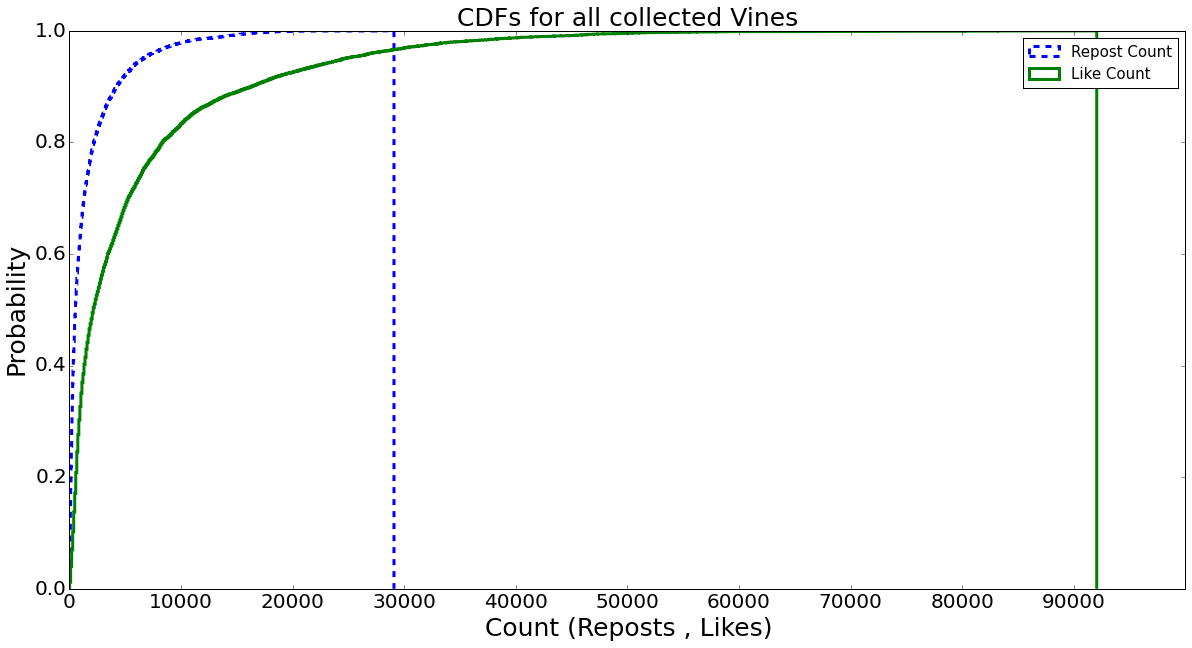
\includegraphics[width=\columnwidth]{plots/Like_repost_CDF}
\caption{\textbf{CDF of likes and repost count across collected Vines.}}
\label{fig:Like_Repost_CDF}
\end{figure}

Figure \ref{fig:Like_Repost_CDF} shows that the behaviour of reposts could be used as a viable metric for user's interaction with a vine video and dissemination of the video in the network. 

\begin{figure}
\centering
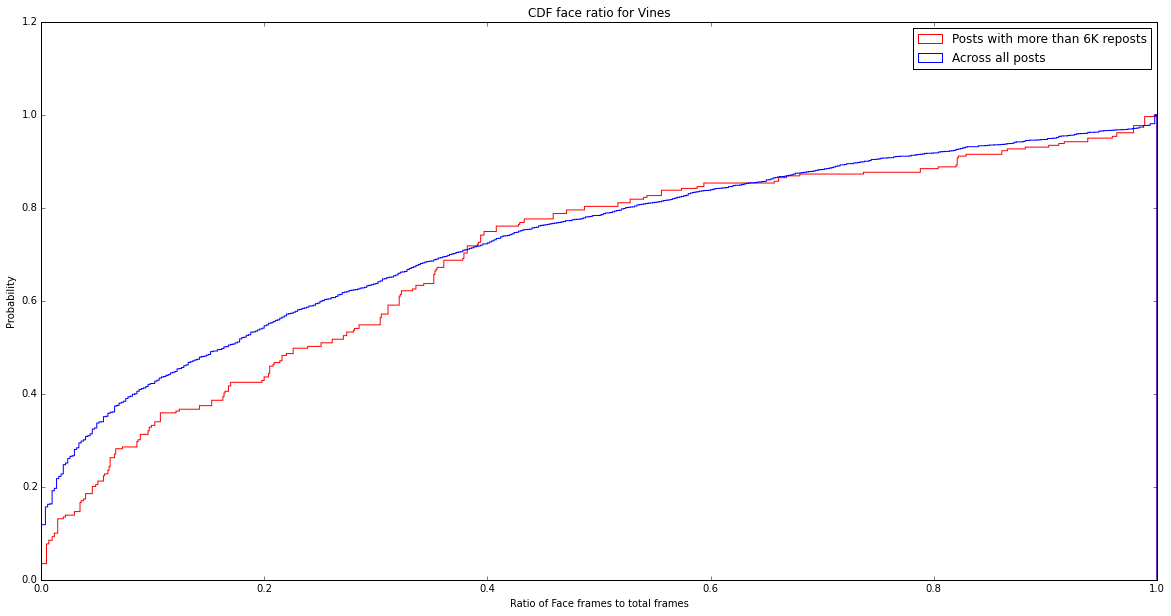
\includegraphics[width=\columnwidth]{plots/CDF_Compound}
\caption{\textbf{CDF of Face frames to total frames calculated for Frontal and Profile faces }}
\label{fig:Like_Repost_CDF}
\end{figure}

\begin{figure}
\centering
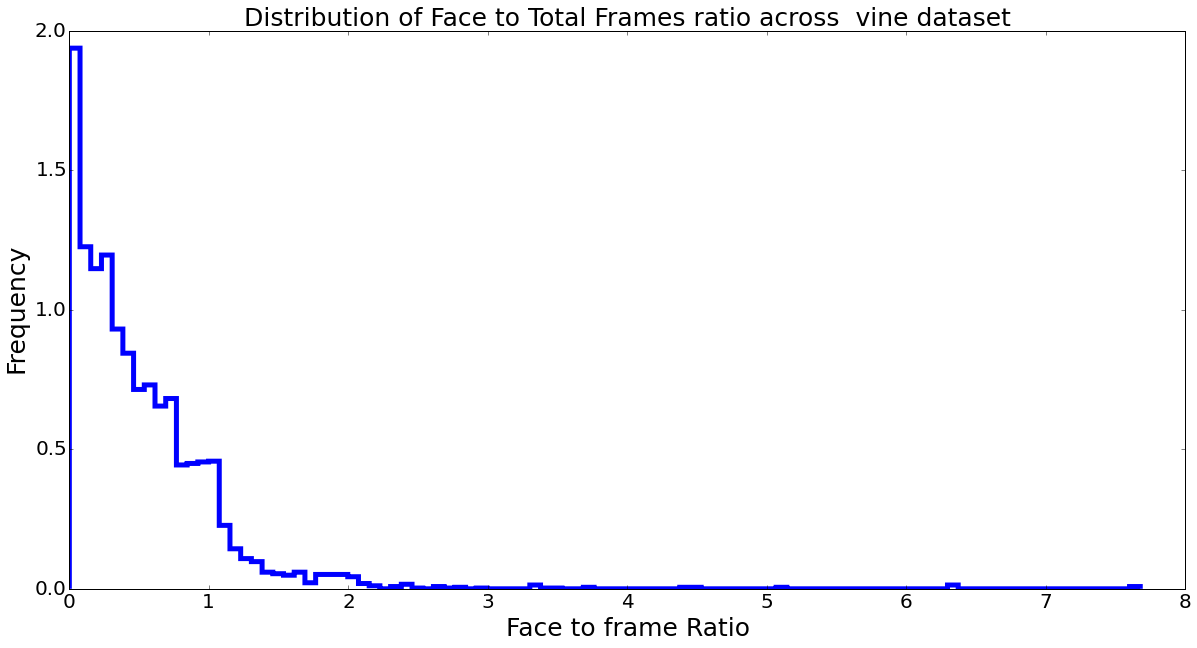
\includegraphics[width=\columnwidth]{plots/faceratio_destribution_dataset}
\caption{\textbf{ Distribution of face frames compared to total frames for all the Vine videos in the dataset}}
\label{fig:Like_Repost_CDF}
\end{figure}
